\documentclass[%>>>
     fontsize=11pt%
    %,twoside%
    ,ngerman%
    ,paper=a4%
    ,toc=listof%
    ,toc=bib%
    ,BCOR=3mm%
    ,DIV=13%
    ,open=any% ,capMBOM 651tions=tableabove% ,headings=normal%
]{scrreprt}%<<<


\includeonly{
    ./Talente/talente,
    ./Kampf/Home/home,
    ./Kampf/Angriff/angriff,
    ./Kampf/Parade/parade,
    ./Kampf/Ausweichen/ausweichen,
    ./Kampf/Schaden/schaden,
    ./Kampf/Aktionen/aktionen,
    ./Kampf/Patzer/patzer,
    ./Kampf/Passierschlag/passierschlag,
    ./Kampf/Krit/krit,
    ./Kampf/Waffenlos/waffenlos,
}


% Packages >>>
\usepackage[utf8]{inputenc}      % usage of most utf8 characters on input
\usepackage[T1]{fontenc}         % usage of correct font encoding for Umlauts
\usepackage{lmodern}             % scalable and slightly better looking font
\usepackage{amsmath}             % mathematics
%\usepackage{mathtools}           % useful stuff for spacing etc.
\usepackage{graphicx}            % easy include of images
\usepackage{float}
\usepackage{booktabs}            % prettier tables
\usepackage[table]{xcolor}       % easy to use coloring
%\usepackage{multirow}            % more than one row in a table column
\usepackage{longtable}           % page breakable tables
\usepackage{collcell}            % make a cell the argument of a command
\usepackage{array}               % cool stuff for tables and the like
\usepackage{placeins}            % better control over placement of figures
\usepackage{csquotes}            % to silence biblatex's warnings concerning it
\usepackage{scrlayer-scrpage}    % page header and footer configuration >>>
\usepackage{pdfpages}
\usepackage{multicol}
\usepackage{wrapfig}
\usepackage{tikz-qtree}
\setlength{\columnsep}{1cm}
    \KOMAoptions{%
        ,headsepline=true%
        ,headinclude=true%
        %,headlines=2%
    }
    \setkomafont{pageheadfoot}{\sffamily}
    \ihead*{\headmark}
    \chead*{}
    \ohead*{DSA Flowcharts}
    \ifoot*{}
    \cfoot*{}
    \ofoot*{\pagemark}
    \pagestyle{scrheadings}
    \renewcommand*{\chapterpagestyle}{scrheadings}
    \automark[chapter]{chapter} % both right and left chapters
    %\automark*[section]{} % if there is a section right head containing section
\usepackage[% babel >>>          % German language
    main=ngerman%
    ,english%
]{babel}%<<<
\usepackage{pgf}                 % plots
\usepackage{xparse}              % better/easier macro creation
\usepackage{setspace}            % consistent spacing
\usepackage[export]{adjustbox}
\usepackage{multicol}
\usepackage{tabularx}
\usepackage{tabulary}
\usepackage{siunitx}             % consistent units and numbers formatting
\usepackage{wrapfig}
\usepackage{microtype}
\usepackage{framed}
\usepackage{enumitem}
\usepackage[pdftex,pdfpagelabels,bookmarks,hyperindex,hyperfigures]{hyperref}
\usepackage{lipsum}
\usepackage{xparse}
%<<<

\NewDocumentCommand\ts{ O{} m }{_{#1\text{#2}}}%
\newtheorem{defi}{Definition}[section]
\newcommand{\laplace}{\Delta}
\setcounter{tocdepth}{5}

\setlength{\parindent}{0pt}
\setlength{\parskip}{\baselineskip}
\setlist{itemsep=0pt,parsep=0pt}

\newcommand{\fett}[2]{\textbf{\textit{{\color{#1}#2 }}}}
\newcommand{\fetts}[1]{\textbf{\textit{{\color{blue}#1 }}}}
\newcommand{\comm}[1]{
\begin{leftbar}
	#1
\end{leftbar}
}
\newcommand{\ggline}[2]{\textbf{#1} & \multicolumn{6}{l}{#2}\\}

\newcommand{\fmip}[1]{
  \begin{fminipage}{\textwidth}
	#1
\end{fminipage}
}
\newcommand{\parline}[1]{\paragraph{#1}\mbox{}\\}
\newcommand{\subparline}[1]{\subparagraph{\fetts{#1}}\mbox{}\\}
\newcommand{\hylin}[2]{\hyperlink{#1}{\color{red}\textbf{#2}}}
\newcommand{\hylt}[3]{\hypertarget{#1}{\hylin{#2}{#3}}}
\newcommand{\spp}[2]{
\noindent
\begin{minipage}[t]{.45\textwidth}
    \vspace{0pt}
    #1
\end{minipage}
\hfill\vline\hfill
\begin{minipage}[t]{.45\textwidth}
    \vspace{0pt}
    \raggedleft
    #2
\end{minipage}
}

\newcommand{\pers}[5]{
    \comm{
    \fetts{#1}

    \textit{\underline{Erscheinung}:} #2 

    \textit{\underline{Charakter}:} #3 

    \textit{\underline{Darstellung}:} #4 

    \textit{\underline{Weiteres}:} #5 
    }
}



\newsavebox{\fminipagebox}
\NewDocumentEnvironment{fminipage}{m O{\fboxsep}}
{\par\kern#2\noindent\begin{lrbox}{\fminipagebox}
		\begin{minipage}{#1}\ignorespaces}
		{\end{minipage}\end{lrbox}%
	\makebox[#1]{%
		\kern\dimexpr-\fboxsep-\fboxrule\relax
		\fbox{\usebox{\fminipagebox}}%
		\kern\dimexpr-\fboxsep-\fboxrule\relax
	}\par\kern#2
}

\usepackage{tikz}
\usetikzlibrary{positioning}
\usetikzlibrary{shapes,arrows}
\tikzstyle{decision} = [diamond, draw, fill=blue!20, 
    text width=4.5em, text badly centered, node distance=3cm, inner sep=0pt]
\tikzstyle{block} = [rectangle, draw, fill=blue!20, 
    text width=5em, text centered, rounded corners, minimum height=4em]
\tikzstyle{line} = [draw, -latex']
\tikzstyle{cloud} = [draw, ellipse,fill=red!20, node distance=3cm,
    minimum height=2em]


\begin{document}
\chapter{Einleitung}
Cheatsheet Sammlung und Flussdiagramme für wichtige Abläufe in DSA.
    \chapter{Talente}
\section{Heilkunde Wunden}
\begin{minipage}{\textwidth}
    \begin{center}
        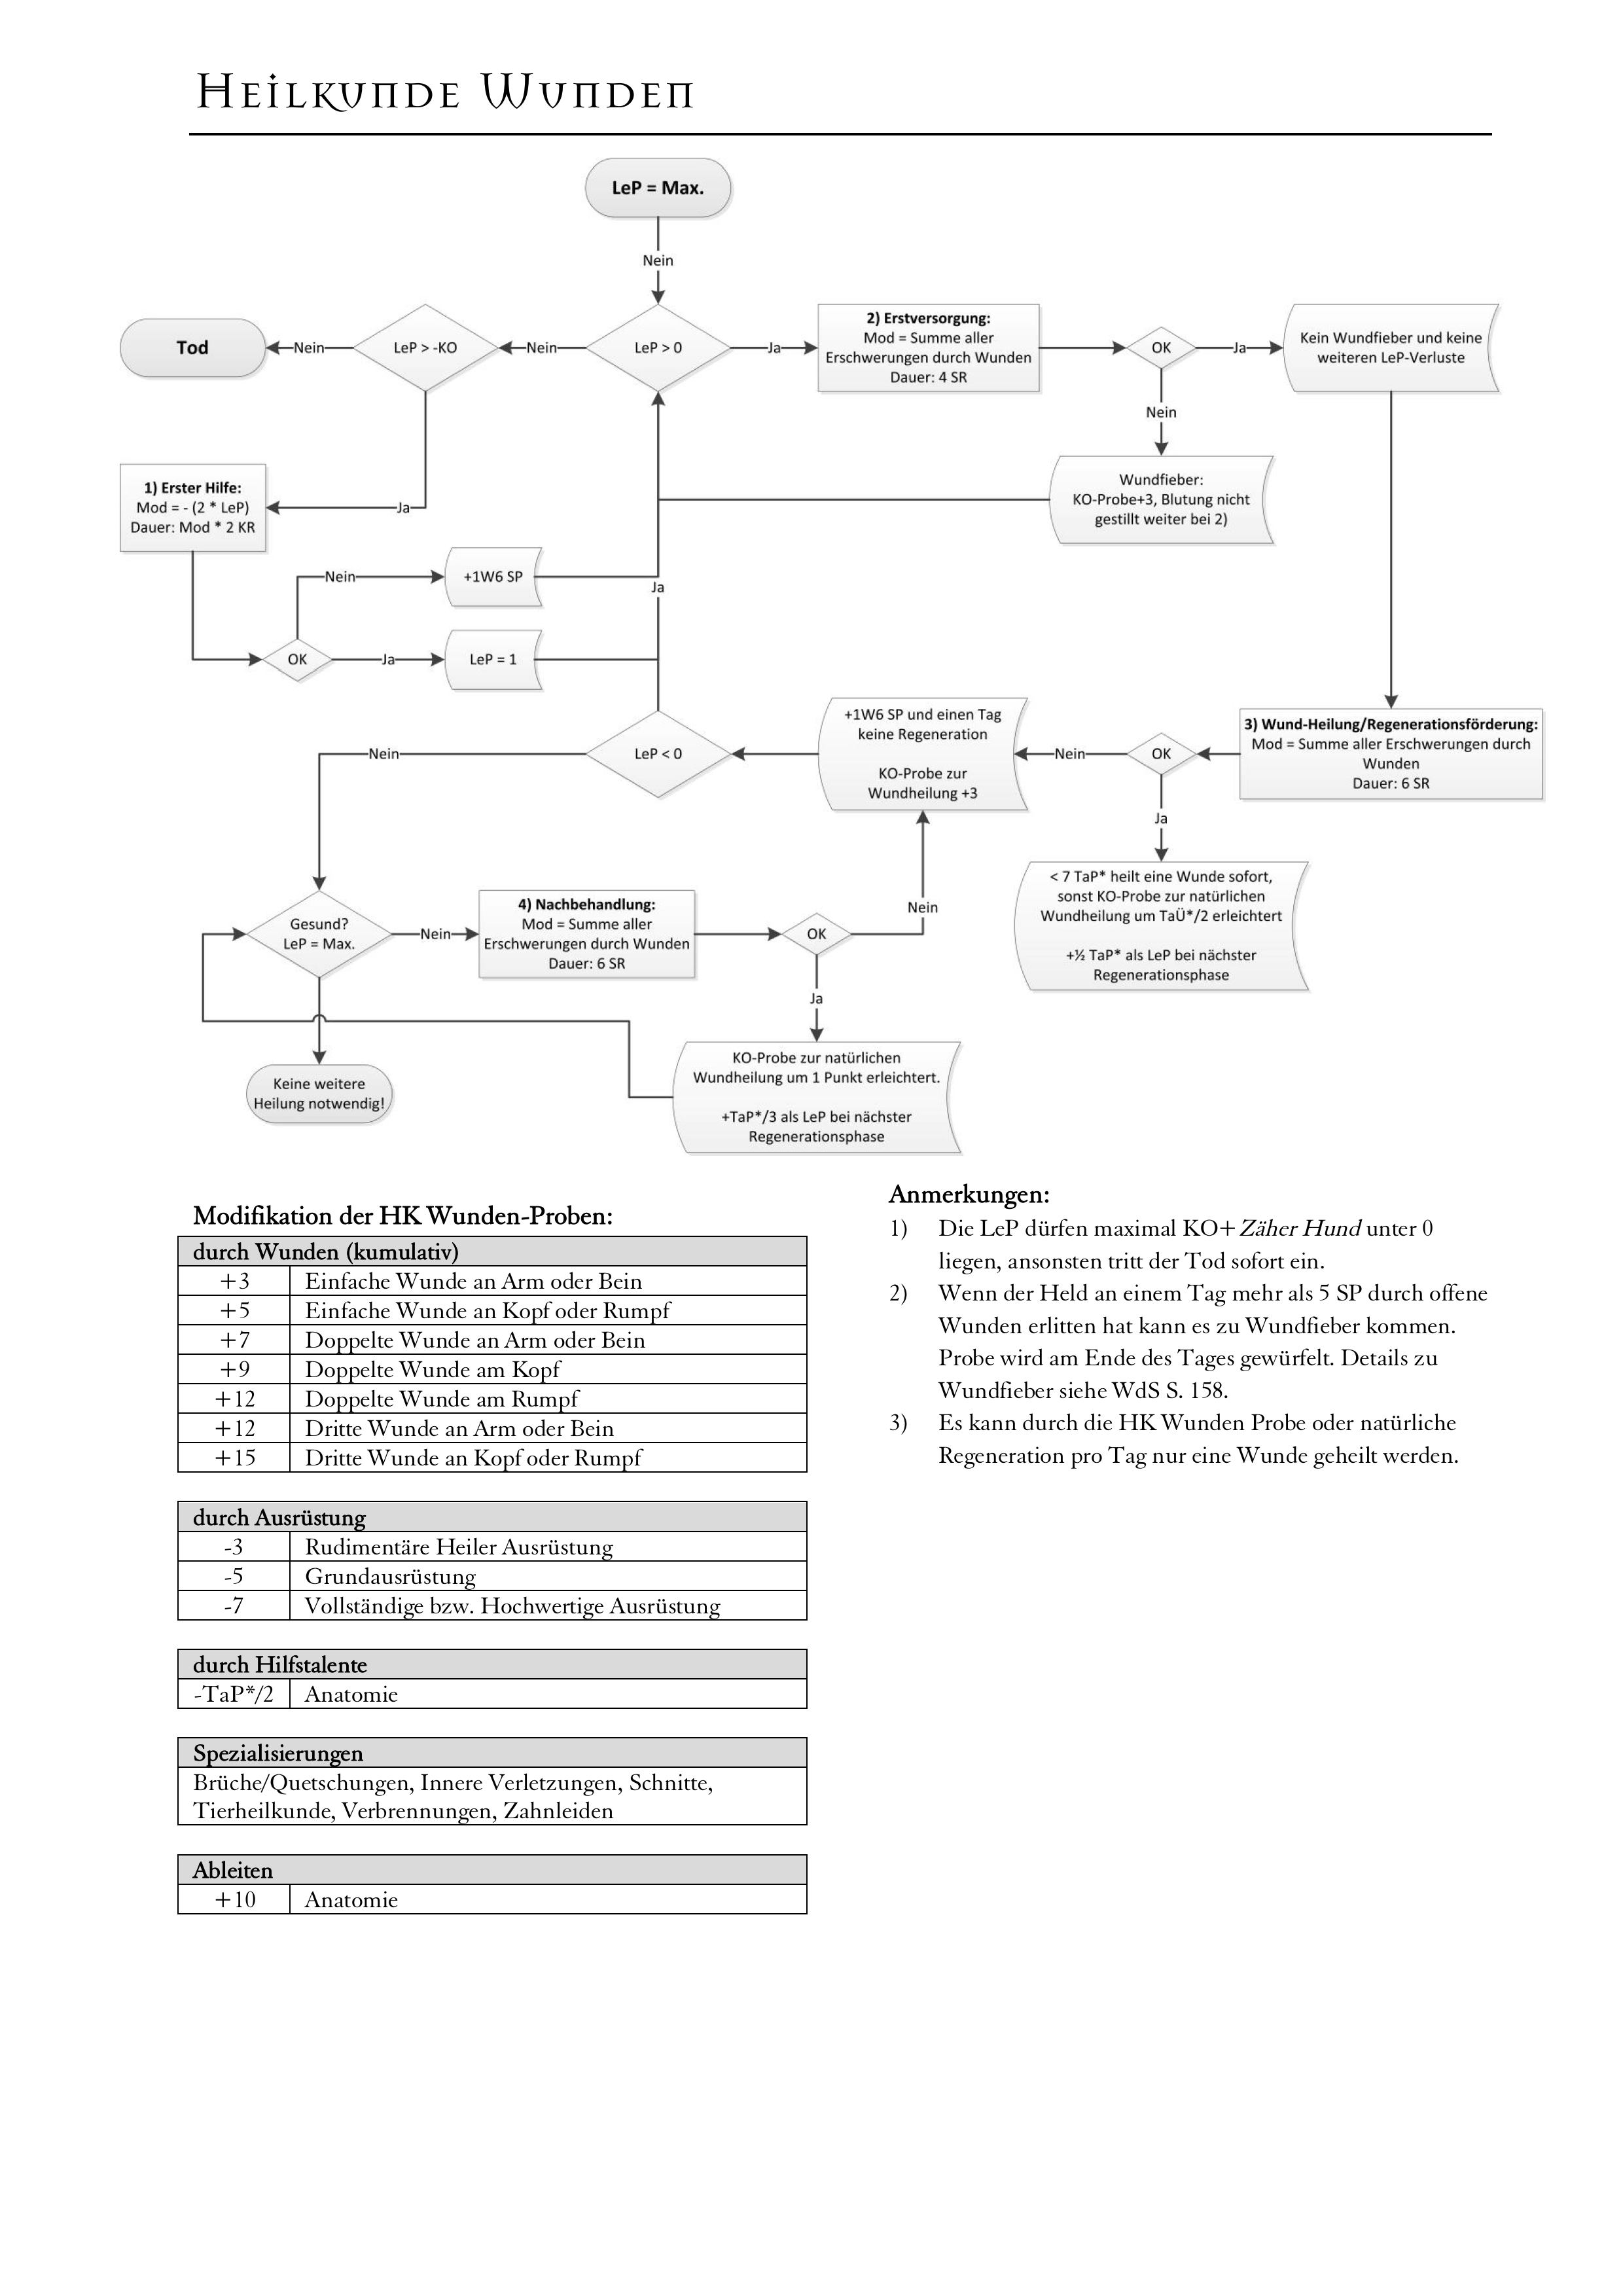
\includegraphics[width=0.7\linewidth,height=0.7\textheight, keepaspectratio]{Talente/HeilkundeWunden/HK-Wunden.png}
    \end{center}
\end{minipage}
\section{Athletik}


    \chapter{Kampfablauf}
\spp{
\section{Kampfbeginn}
\begin{center}
    \begin{tikzpicture}[node distance = 3cm, auto]
            % Nodes
        \node [cloud] (init) {Start} ;
        \node [block, below of=init] (initiative) {\hypertarget{initiativestart}{\hylin{initiative}{Initiative}}};
        \node [block, below of=initiative] (ansage) {Ansage von niedrigster Initiative an};
        \node [block, right of=ansage] (hinweis) {Manöver mit 2 Aktionen nicht umwandelbar};
        \node [block, below of=ansage] (ausf) {Ausführung von höchster Initiative an};
        \node [block, below of=ausf] (angr) {\hypertarget{angriffstart}{\hylin{angriff}{Angriff}}};
        \node [block, below of=angr] (par) {\hylt{paradestart}{parade}{Parade}};
            % Edges
        \path [line] (init) -> (initiative);
        \path [line] (initiative) -> (ansage);
        \path [line] (ansage) -> (ausf);
        \path [line] (ausf) -> (angr);
        \path [line] (angr) -> (par);
    \end{tikzpicture}
\end{center}
}{
    \section{Ablauf eines Initiativeschritts}
    \begin{center}
        \begin{tikzpicture}[node distance = 3cm, auto]
                % Nodes
            \node [cloud] (init) {Du bist dran};
            \node [decision, below of=init] (aufmerk) {Aufm.?};
            \node [decision, below left of=aufmerk] (ans) {Abwar.?};
            \node [block, below left of=ans] (abw) {\hylin{abwarten}{Abwarten}};
            \node [block, below right of=ans] (aend) {Ansage ändern};
            \node [block, below of=aend] (ausf) {Ausführen};
            \node [below right = 0.5cm of aufmerk] (no) {Nein};
                % Edges
            \path [line] (init) -- (aufmerk);
            \path [line] (aufmerk) --node[above left] {Ja} (ans);
            \path [line] (ans) --node[above left] {Ja} (abw);
            \draw [line] (aufmerk) to [bend left=40] (ausf);
            \path [line] (ans) --node[above right] {Nein} (aend);
            \path [line] (aend) -- (ausf);
        \end{tikzpicture}
    \end{center}
}
\newpage
\section{Initiative / Hinterhalt}
\begin{minipage}[t]{\linewidth}
\begin{center}
    \begin{tikzpicture}[node distance = 3cm, auto]
            % Nodes
        \node [cloud] (init) {\hypertarget{initiative}{\hylin{initiativestart}{Initiative}}} ;
        \node [decision, below of=init] (surpr) {Überrascht};
        \node [decision, below left of=surpr] (surprja) {Hinterhalt};
        \node [block, below right of=surpr] (surprno) {Initiative Wurf};
        \node [block, below right of=surprja] (hintno) {\textbf{IN}/KR für Ini Wurf*};
        \node [block, below left of=surprja] (hintja) {Freie Handlung f. Angreifenden};
        \node [block, below of=hintja] (hintausw) {\textbf{IN}(+3 bei Fernkampf) zum Parieren/Ausw.};
            % Edges
        \path [line] (init) -- (surpr);
        \path [line] (surpr) -- node[above left] {Ja} (surprja);
        \path [line] (surpr) -- node {Nein} (surprno);
        \path [line] (surprja) -- node {Nein} (hintno);
        \path [line] (surprja) -- node[above left] {Ja} (hintja);
        \path [line] (hintja) -- (hintausw);
        \draw [line]    (hintausw) to[out=0,in=-90] (hintno);
    \end{tikzpicture}
\end{center}
\end{minipage}
\spp{
    \begin{center}
        \begin{tabularx}{\linewidth}{|c|X|}
            \multicolumn{2}{l}{\textbf{*)} Erleichterungen der Probe zu KR Beginn}\\
            \hline
           -1 / 2 TaP &  \textit{Kriegskunst}, \textit{Gefahreninstinkt}\\
           \hline
           -4 & \textit{Aufmerksamkeit}, \textit{Kampfgespür}\\
           \hline
        \end{tabularx}
    \end{center}
}{
    Auf Aktion \textit{Waffe ziehen} achten!
}
    \chapter{Nahkampfangriff}
\spp{
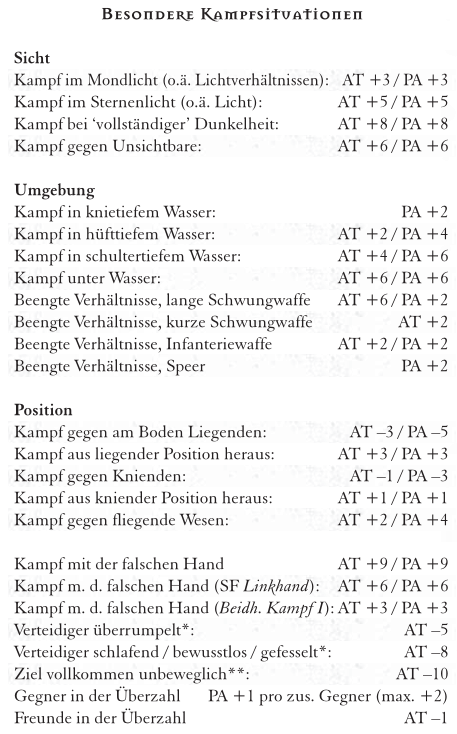
\includegraphics[width=.9\linewidth]{Kampf/Home/kampfsituationen.png}\\
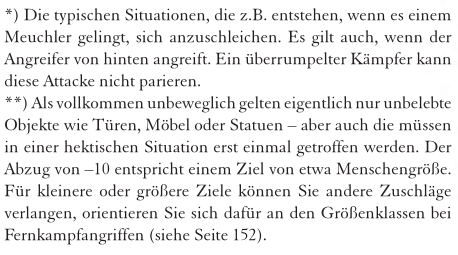
\includegraphics[width=.9\linewidth]{Kampf/Home/kampfsituationenkommentar.png}
}{
\begin{center}
    \begin{tikzpicture}[node distance = 2cm, auto]
            % Nodes
        \node [block] (init) {\hylt{angriff}{angriffstart}{Angriff}} ;
        \node [block, below of=init] (man) {Manöver wählen:\\\hylin{angriffskarten}{NK} / \hylin{fernkampfkarten}{FK}};
        \node [block, below of=man] (erschw) {Erschwernis};
        \node [decision, below =0.3cm of erschw] (par) {\hylt{paradeangr}{parade}{Pariert?}};
        \node [block, below of=par] (end) {\hylin{schaden}{Treffer}};

            % Edges
        \path [line] (init) -> (man);
        \path [line] (man) -> (erschw);
        \path [line] (erschw) -> (par);
        \path [line] (par) -> (end);
    \end{tikzpicture}
\end{center}
\begin{center}
    \begin{tabular}{| c | l |}
        \hline
        \textbf{Zone }& \textbf{Erschwernis}\\
        \hline
        Kopf & +4\\
        \hline
        Brust & +6\\
        \hline
        Arme**& +4/+6\\
        \hline
        Bauch & +4\\
        \hline
        Beine & +2\\
        \hline
    \end{tabular}
\end{center}
\textbf{Gezielter Schlag:} Zonenerschwernis nochmal +2. Kombinierbar mit Finte oder Wuchtschlag

\textbf{Gezielter Stich/Todesstoß auf Zone:} halbe Zonenerschwernis.}
Die \textbf{zweite Angriffsaktion} (umgewandelt) findet \textbf{8} Initiativepunkte \textbf{nach} der Initiative des Akteurs statt.

\textbf{Ansage:} Freiwillige \underline{\textit{plus}} geforderte Erschwernis.

Misslingen: \textbf{nächste} Aktion um gesamte \textbf{Ansage} erschwert.

\chapter{Fernkampfangriff}
\spp{
\begin{center}
    \begin{tikzpicture}[node distance = 3cm, auto]
            % Nodes
        \node [cloud] (init) {\hypertarget{fernkampf}{\textbf{FK} Angriff (Waffe besehnt)}} ;
        \node [decision, below of=init] (atk) {Schnell.?};
        \node [block, below left of=atk] (ssja) {Erschw. +2 (+0 Meist. schütz.)};
        % \node [block, below right = 1cm of ssja] (schuss) {Erschw. n. Tab.};
        \node [decision, right of=atk] (ssno) {Ansage / Zielen / Schießen?};
        \node [block, below right = 2cm of ssno] (ans) {+1 Akt / 2 Ansagepkt.*};
        \node [block, below of=ssno] (ziel) {Erschw. -1(max 4) / 2 Akt.};
        \node [block, below of=ans] (ansdmg) {TP + Ansagepkt./2**};
        \node [block, below left = 2cm of ansdmg] (schuss) {Erschw. nach Tabelle};
            % Edges
        \path [line] (init) -- (atk);
        \path [line] (atk) -- node[above left] {Ja} (ssja);
        \path [line] (atk) -- node {Nein} (ssno);
    \end{tikzpicture}
\end{center}
\begin{center}
    \begin{tabularx}{\linewidth}{cX}
        \hline
        \textbf{*)} & Ansage <=TaW; Meisterschütze: <= \textbf{FK}\\
        \hline
        \textbf{**)} & \textit{Scharfschütze} darf ganze Ansage addieren. 2 Akt. weniger, mind. 1. \textit{Meisterschütze} immer nur 1 Akt.\\
        \hline
    \end{tabularx}
\end{center}
()
}{

}
    \chapter{Parade}
\spp{
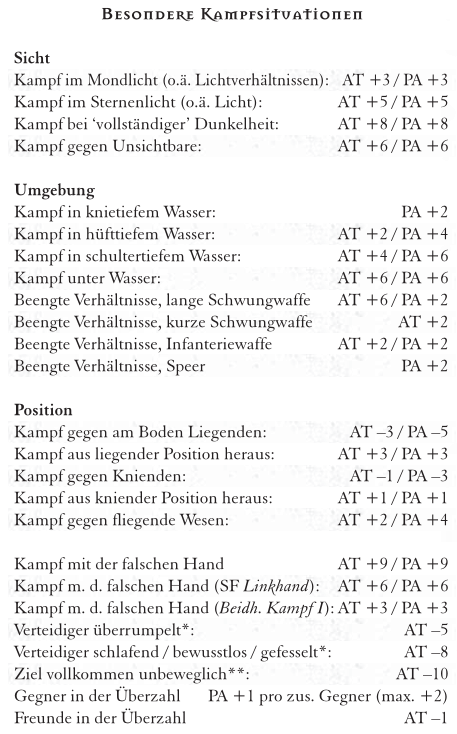
\includegraphics[width=0.9\linewidth]{Kampf/Home/kampfsituationen.png}\\
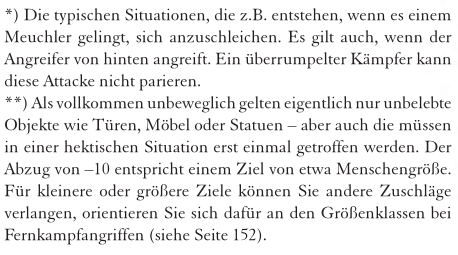
\includegraphics[width=0.9\linewidth]{Kampf/Home/kampfsituationenkommentar.png}
}{
\begin{center}
    \begin{tikzpicture}[node distance = 3cm, auto]
            % Nodes
        \node [block] (init) {\hylt{parade}{paradestart}{Wird angegriffen}} ;
        \node [decision, below of=init] (dec) {Kann parieren?};
        \node [block, right = 1cm of dec] (hit) {\hylin{treffer}{Treffer}};
        \node [decision, below of=dec] (pardec) {Parieren?};
        \node [block, below left of=pardec] (par) {Manöver wählen*:\\\hylin{abwehrkarten}{Parade}};
        \node [block, below right of=pardec] (ausw) {\hylin{ausweichen}{Ausw.}};
        \node [block, below = 3cm of pardec] (end) {\hylin{schaden}{Treffer}};

            % Edges
        \path [line] (init) -> (dec);
        \path [line] (dec) ->node [left] {Ja} (pardec);
        \path [line] (dec) ->node [above] {Nein} (hit);
        \path [line] (pardec) ->node {Nein} (ausw);
        \path [line] (pardec) ->node[above left] {Ja}(par);
        \path [line] (par) -> node[below left] {Nein} (end);
        \path [line] (ausw) -> node[below right] {Nein} (end);
    \end{tikzpicture}\\
\end{center}
*) Einen \textbf{Gezielten Schlag} zu parieren ist um -2 (Bauch/Brust), -4
*(Kopf) erleichtert. Mit \textit{Aufmerksamkeit} um zusätzlich -2.

Eine \textbf{Parade} muss vor auswürfeln der \textbf{Attacke} angesagt
werden. Bei misslingen der Attacke \textbf{verfällt } die Parade. Sonst wäre
reaktives Kämpfen zu stark.
}
    \section{Ausweichen}
\begin{center}
    \begin{tikzpicture}[node distance = 3cm, auto]
            % Nodes
        \node [block] (init) {\hypertarget{ausweichen}{Wird angegriffen}} ;
        \node [decision, below of=init] (erschw) {Gezielt Ausw.? (Ausw. I nötig)};
        \node [decision, below left = 3cm of erschw] (gezielt) {Erschw. aus DK x2};
        \node [block, below left of=gezielt] (bestanden) {Entgeht Angriff};
        \node [block, below right of=gezielt] (verkackt) {Wird getroffen, INI -2};
        \node [decision, below right = 3cm of erschw] (ungezielt) {Erschw.};
        \node [block, below left of=ungezielt] (bestanden2) {Entgeht Angriff, INI -4, \textit{Position}};
        \node [block, below right of=ungezielt] (verkackt2) {Wird getroffen, INI -4, \textit{Position}};

            % Edges
        \path [line] (init) -> (erschw);
        \path [line] (erschw) -> (gezielt);
        \path [line] (gezielt) -> (bestanden);
        \path [line] (gezielt) -> (verkackt);
        \path [line] (erschw) -> (ungezielt);
        \path [line] (ungezielt) -> (bestanden2);
        \path [line] (ungezielt) -> (verkackt2);
    \end{tikzpicture}\\
\end{center}
\begin{center}
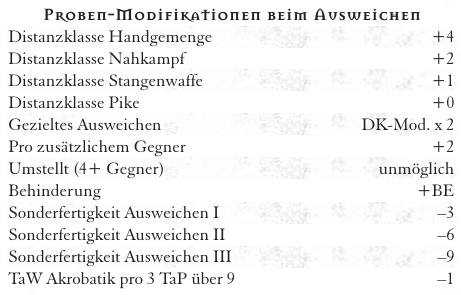
\includegraphics[width=\linewidth]{Kampf/Ausweichen/img/erschwernis.png}
\end{center}
    \chapter{Schaden / Wunden}
\spp{
    *) \textit{Eisern} / \textit{Glasknochen}: -2/+2\\
    **) Bei steifen Rüstungen (Eisen, auch beschlagene Teile!)\\
    ***) +8/+12 bei 2/3 Wunden gleichzeitig. Es wird nur EINMAL gewürfelt.\\
\begin{center}
    \begin{tabularx}{\linewidth}{ccXX}
        \hline
        \textbf{Zone} & \textbf{W20} & \textbf{Erste \& Zweite Wunde} & \textbf{Dritte Wunde}\\
        \hline
        Kopf & 19-20 & MU, KL, IN, INI-Basis -2, INI -2W6 & +2W6 SP,  bewusstlos, Blutverlust\\
        \hline
        Brust & 15-18 & AT, PA, KO, KK-1; +1W6 SP & bewuswstlos, Blutverlust\\
        \hline
        Arme* & 9-14 & AT, PA, KK, FF -2 mit diesem Arm & Arm handlungsunfähig\\
        \hline
        Bauch & 7-8 & AT, PA, KO, KK, GS, INI-Basis -1; +1W6 SP & bewusstlos, Blutverlust\\
        \hline
        Beine* & 1-6 & AT; PA, GE, INI-Basis -2; GS -1 & Sturz, kampfunfähig\\
        \hline
        \multicolumn{4}{l}{*) Ungerade: Schildarm, Gerade: Schwertarm}
    \end{tabularx}
    \textbf{Keine Neuberechnung} der AT, PA, FK und INI-Basiswerte!
\end{center}
}{
\begin{center}
    \begin{tikzpicture}[node distance = 3cm, auto]
            % Nodes
        \node [block] (init) {\hypertarget{schaden}{Wird getroffen}};
        \node [block, below  of=init] (zone) {Zone würfeln};
        \node [block, below of=zone] (rs) {RS verrechnen};
        \node [decision, below of=rs] (dec) {SP > KO/2?*};
        \node [decision, below left of=dec] (wunde) {\textit{Selbstbeh.} + (SP-KO/2)};
        \node [block, below left of=wunde] (ko){1W6+3 KR kampfunfähig};
        \node [decision, below right of=wunde] (kons) {\textit{Selbstbeh.} + 4***};
        \node [block, below right of=dec] (lep) {LeP sinken um SP};
        \node [block, below right of=kons] (abz) {Auswirkung der Wunde, LeP sinken um SP};

        \node [block, right of=zone] (dmg) {\textbf{TP} > 20?};
        \node [block, below of=dmg] (end) {BE der Rüstung steigt um 1**};

            % Edges
            \path [line] (init) -- (zone);
            \path [line] (zone) -- node {TP} (rs);
            \path [line] (rs) -- node {SP} (dec);
            \path [line] (dec) -- node {Ja} (wunde);
            \path [line] (dec) -- node {Nein} (lep);
            \path [line] (wunde) -- node {Ja} (ko);
            \path [line] (wunde) -- node {Nein} (kons);
            \path [line] (kons) -- node {Ja} (lep);
            \path [line] (kons) -- node {Nein} (abz);

            \path[line] (zone) -- (dmg);
            \path[line] (dmg) -- node {Ja} (end);
    \end{tikzpicture}\\

\end{center}
}
    \chapter{Patzer / Bruchtest}
Der Prüfwurf ist \textbf{genauso} erschwert wie der Originalwurf!\\
\spp{\section{Nahkampf}
\begin{center}
    \begin{tabularx}{\linewidth}{cX}
        \hline
        \textbf{2W6}& \textbf{Auswirkungen}\\
        \hline
        2& \textbf{Waffe zerstört: INI -4}. Bei \textbf{BF} 0 -> gilt als 9-10. Bei Faust/Fuß -> gilt als 12.\\
        \hline
        3-5& \textbf{Sturz: INI -2}. Gilt als \textit{am Boden}. Benötigt
        eine Aktione \textit{Position} und eine \textbf{GE}+BE Probe.
        \textit{Standfest}/\textit{Balance}, wandelt in eine einfache
        \textbf{GE}+BE Probe.\\
        \hline
        6-8& \textbf{Stolpern: INI -2}.\\
        \hline
        9-10& \textbf{Waffe verloren: INI -2}. Waffe wiederfinden: Aktion \textit{Position} und \textbf{GE}. Bei Faust/Fuß -> 3-5.\\
        \hline
        11& \textbf{An eigener Waffe verletzt: INI -3}. Waffenschaden (ohne TP/KK oder Ansage) inkl. Wunden falls über KO/2 SP.\\
        \hline
        12& \textbf{Schwerer Eigentreffer: INI -4}. Doppelter Waffenschaden (ohne TP/KK oder Ansage) inkl. Wunden.\\
        \hline
    \end{tabularx}\\
\end{center}
\subsection{Patzer}
\begin{center}
    \begin{tabularx}{\linewidth}{cX}
        \hline
        \textbf{2W6} & \textbf{Auswirkungen}\\
        \hline
        ans <= BF & Waffe/Schild des Verteidigers zerbricht\\
        \hline
        12 > ans > BF & BF von Waffe/Schild des Verteidigers steigt um 1.\\
        \hline
        ans == 12 & BF von Waffe/Schild des Verteidigers unverändert; Angreifer muss Bruchtest ablegen.\\
        \hline
    \end{tabularx}
\end{center}
}{\section{Fernkampf}

\begin{center}
    \begin{tabularx}{\linewidth}{cX}
        \hline
        \textbf{2W6}& \textbf{Auswirkungen}\\
        \hline
        2& \textbf{Waffe zerstört: INI -4}. Hässliches Knacken, Waffe so schwer
        beschädigt, dass Reparatur nicht lohnt. \textbf{Schütze verliert alle
        verbleibenden Aktionen dieser Runde.}\\
        \hline
        3& \textbf{Waffe beschädigt: INI -3}. Projektil landet vor Füßen des
        Schützen. Sehne ist gerissen, Armbrust ernsthaft verklemmt.
        \textbf{Schütze verliert alle verbleibenden Aktionen dieser Runde.}\\
        \hline
        4-10& \textbf{Fehlschuss: INI -2}. Schütze benötigt \textbf{2 Aktionen} um Waffe wieder schussfähig zu machen.\\
        \hline
        11-12& \textbf{Kamerade getroffen: INI -3}. Der Schuss löst sich
        unbeabwsichtigt. Trifft den nächsten Helden in der Schussbahn.
        \textbf{Ansagen} kommen nicht zum tragen beim Schaden. \textbf{Ist
        kein Held in der nähe, hat Schütze sich selbst verletzt.} (TP gemäß
        geringster Entfernung.)\\
        \hline
    \end{tabularx}
\end{center}
}
    \chapter{Passierschlag}
\hypertarget{passierschlag}{}
\begin{center}
    \begin{tikzpicture}[node distance = 3cm, auto]
        \node [block] (init) {Gegner bewegt sich in / durch \textit{Kontrollbereich*}};
        \node [decision, below of=init] (dec1) {Test**};
        \node [block, below left of=dec1] (schlag) {Attacke +4***};
        \node [block, right = 2cm of schlag] (miss) {Gegner passiert};
        \node [block, below of=schlag] (end) {TP \textit{und} -1W6 INI für Gegner};
        % edges
        \path [line] (init) -- (dec1);
        \path [line] (dec1) --node[above left] {Ja} (schlag);
        \path [line] (dec1) --node {Nein} (miss);
        \path [line] (schlag) --node[left] {Ja} (end);
        \path [line] (schlag) --node[above] {Nein} (miss);
        \path [line] (end) -- (miss);
    \end{tikzpicture}
\end{center}
\textbf{*)} Bereich von 3 Feldern \textbf{VOR} Kämpfer.

\textbf{**)} Gegner ignoriert Kämpfer \textit{und} Kämpfer ist nicht mit
\textbf{längerfristiger Aktion} beschäftigt oder in \textbf{Unterzahl}.

\textbf{***)} -WM der \textbf{Waffe die Passierschlag ausführt} auf Attacke-Modifikator. Gegen Opfer mit \textit{Aufmerksamkeit} um zusätzlich +4.
    \chapter{Kritische Treffer}

\begin{center}
    \begin{tikzpicture}[node distance = 3cm, auto]
        % nodes
        \node [block] (init) {\textbf{1} bei Attackewurf};
        \node [decision, below of=init] (par) {Parade / Ausw. mit \textbf{halbem} Wert!*};
        \node [block, below left of=par] (pariert) {Angriff pariert.};
        \node [decision, below right = 2cm of par] (hit) {Angriff bestätigen**};
        \node [block, below right of=hit] (unbes) {Normaler Treffer};
        \node [block, below left of=hit] (schaden) {Schaden erhöhen***};
        % edges
        \path [line] (init) -- (par);
        \path [line] (par) --node{Nein}(hit);
        \path [line] (par) --node[above left]{Ja}(pariert);
        \path [line] (hit) --node[above left]{Ja}(schaden);
        \path [line] (hit) --node{Nein}(unbes);
    \end{tikzpicture}
\end{center}
\textbf{*)} Erschwernisse durch fehlgeschlagene Manöver oder Finten erst
\textbf{nach} Halbierung verrechnen.

\textbf{**)} Bestätigungswurf ist \textbf{genauso} erschwert wie der normale Angriff!

\textbf{***)} Verdopplung der \textbf{Waffenschadenspunkte}, keine
Verdopplung von Ansagen oder TP/KK. Zählt immer nur der höchste Modifikator
(\textbf{Hammerschlag} trotzdem nur x3)!
    \chapter{Waffenlose Manöver / Freie Aktionen}
\spp{
    \section{Waffenlose Manöver für Jedermann}
\begin{itemize}
    \item Biss
    \item Block
    \item Fußfeger +3
    \item Gerade/Tritt
    \item Griff
    \item Knaufschlag
    \item Knie
    \item Kopfstoß
    \item Niederringen
    \item Schmutzige Tricks + \textbf{IN} Probe
    \item Schwinger
    \item Sprungtritt (wenn \textbf{BE} / Umstände es zulassen)
\end{itemize}
}{
\section{Freie Aktionen}
\begin{itemize}
    \item Aktivierung eines am Körper getragenen oder in der Hand gehaltenen magischen Artefakts
    \item \hylin{ausweichen}{Ausweichen}
    \item Drehen ($45^\circ$ Drehung)
    \item \hylin{passierschlag}{Passierschlag}
    \item Rufen (3 \textbf{kurze} Worte)
    \item Schritt (Verändert \textbf{nicht} die DK)
    \item Sich zu Boden werfen (\textbf{GE} :- -1W6 INI)
    \item Waffe oder Gegenstand fallen lassen (heißt \textbf{nicht} vorsichtig absetzen!)
\end{itemize}
Freie Aktion zu jedem Zeitpunkt ausführbar. Nur \textbf{eine} Aktion pro
Initiativabschnitt pro Person durchführbar. Bei \textbf{mehreren} Freien
Aktionen \textbf{unterschiedlicher} Akteure im selben Initiativabschnitt,
entscheidet die Initiative der Akteure wessen Aktion zuerst durchgeführt wird.

\textbf{Ein Initiativeabschnitt} ist ein 'Feld' auf dem Initiative-'Zeitstrahl'.
}
    \chapter{Aktionen}
\spp{
\section{Abwarten}
\hypertarget{abwarten}{}
Man muss unterscheiden zwischen \textit{verzögern} und \textit{abwarten}.

\textbf{Abwarten} kann \textit{nur} derjenige mit der höheren INI. Sollten beide Parteien eines Zweikampfes verzögern:

In dem Fall nehmen beide ihre aufgesparte Aktion mit in die nächste Runde, zu
Beginn der Runde (also noch bevor einer der beiden mit der INI dran ist)
attackiert derjenige mit der höheren INI (muss er natürlich nicht, aber
jedenfalls ist dies die kluge Vorgehensweise). Der mit der niedrigeren INI
kann sich dann entscheiden seine aufgesparte Aktion zu verlieren und seine
Parade dieser Runde zu verwenden oder er kriegt einen unparierbaren Angriff,
wenn der trifft muss er eine \textit{Selbstbeherrschungs}-Probe + SP hinlegen oder er
\textbf{verliert} seine aufgesparte Aktion.

\mbox{}
\vfill
\hline
\mbox{}
\vfill
\textbf{*)} Ausführender selbst zählt \textbf{nicht} als Beteiligter!

\textbf{**)} Freiwillig um doppelte Überzahl der Gegner erschwert, dann fällt Überzahlbonus weg.

\textbf{***)} Max. 6 auf INI Werte der Beteiligten (\textbf{nicht} er selbst), wenn \textbf{positiver} Kriegskunstwert.
}{
    \section{Taktik}
    \textbf{Einmal} pro KR und einmalig pro Beteiligtem!
\begin{center}
    \begin{tikzpicture}[node distance = 2cm, auto]
            % Nodes
        \node [block] (init) {Anführer (höchste Kriegskunst)};
        \node [decision, below of=init] (ueberr) {Überra.?};
        \node [right of=ueberr] {Nein};
        \node [block, below = 1cm of ueberr] (in) {Erst nach \textbf{IN} Probe};
        \node [block, below of=in] (dec) {Festlegen der Beteiligten *};
        \node [decision, below of=dec] (kk) {\textit{Kriegskunst} Probe**};
        \node [block, below left = 1cm of kk] (jo) {\textbf{TaP*} gleichmäßig ***};
        \node [block, below right = 1cm of kk] (no) {-1 INI für jeden \textbf{Beteiligten}};
            % Edges
        \path [line] (init) -- (ueberr);
        \path [line] (ueberr) --node[left] {Ja} (in);
        \draw [line] (ueberr) to [bend left=60] (dec);
        \path [line] (in) -- (dec);
        \path [line] (dec) -- (kk);
        \path [line] (kk) --node [above left] {Ja} (jo);
        \path [line] (kk) --node {Nein} (no);
    \end{tikzpicture}
\end{center}
}
\newpage
\section{Meucheln / Betäuben}
Vorraussetzungen: 
\begin{enumerate}
    \item Kommt an Opfer unbemerkt heran (\textit{Schleichen} / \textit{Sich Verstecken})
    \item passende Waffe in der Hand, die \textbf{Opfer nicht bemerkt hat}
    \item Opfer muss \textbf{völlig} ahnungslos sein
\end{enumerate}
\begin{center}
    \begin{tikzpicture}[node distance = 2cm, auto]
            % Nodes
        \node [block] (init) {Opfer ahnungslos};
        \node [block, below of=init] (hit) {Attacke*};
        \node [decision, below of=hit] (vorn) {Von vorne?};
        \node [decision, left of=vorn] (vornjo) {\textbf{IN} Probe Opfer};
        \node [decision, below = 1cm of vornjo] (inpro) {\textit{Raufen}-PA +8};
        \node [block, below = 1cm of vorn] (treffer) {Schaden};
        \node [decision, right = 2cm of treffer] (toeten) {Töten?};
        \node [block, above = 1cm of toeten] (tp) {TP = SP; SP x3**};
        \node [block, right = 1cm of toeten] (bet) {TP = SP(A)};
        \node [decision, above of=bet] (wund) {AU-Verl. > KO/2};
        \node [decision, above of=wund] (wund2) {AU-Verl. > KO};
        \node [block, right = 1cm of wund2] (end) {1W6 SR bewusstlos};
        \node [decision, below = 1cm of end] (prob) {\textbf{KO} + SP(A)};
            % Edges
        \path [line] (init) -- (hit);
        \path [line] (hit) -- (vorn);
        \path [line] (vorn) --node[above] {Ja} (vornjo);
        \path [line] (vorn) --node[right] {Nein} (treffer);
        \path [line] (vornjo) --node[above right] {Nein} (treffer);
        \path [line] (vornjo) --node[left] {Ja} (inpro);
        \path [line] (inpro) --node[above] {Nein} (treffer);
        \path [line] (treffer) -- (toeten);
        \path [line] (toeten) --node[above] {Nein} (bet);
        \path [line] (toeten) --node[left] {Ja} (tp);
        \path [line] (bet) -- (wund);
        \path [line] (wund) --node[left] {Ja} (wund2);
        \path [line] (wund) --node[below] {Nein} (end);
        \path [line] (wund2) --node[above] {Ja} (prob);
        \path [line] (prob) --node[left] {Nein} (end);


    \end{tikzpicture}
\end{center}
\textbf{*)} Je nach Situation um 5 (ahnungslos) bzw. 8 (schläft, bewusstlos,
gefesselt). Mit \textit{Gezielter Stich} um bis zu 8 erschwerbar.
\textit{Anatomie}-Probe: Voller Schaden (wie 6 gewürfelt). Bei
\textbf{Trefferzone} mit \textit{Gezielter Stich} nur halber Aufschlag.

\textbf{**)} Nur mit Dolch, Fechtwaffen und Schwertern möglich.
    \addcontentsline{toc}{chapter}{Angriffsmanöver}
    \hypertarget{angriffskarten}{}
    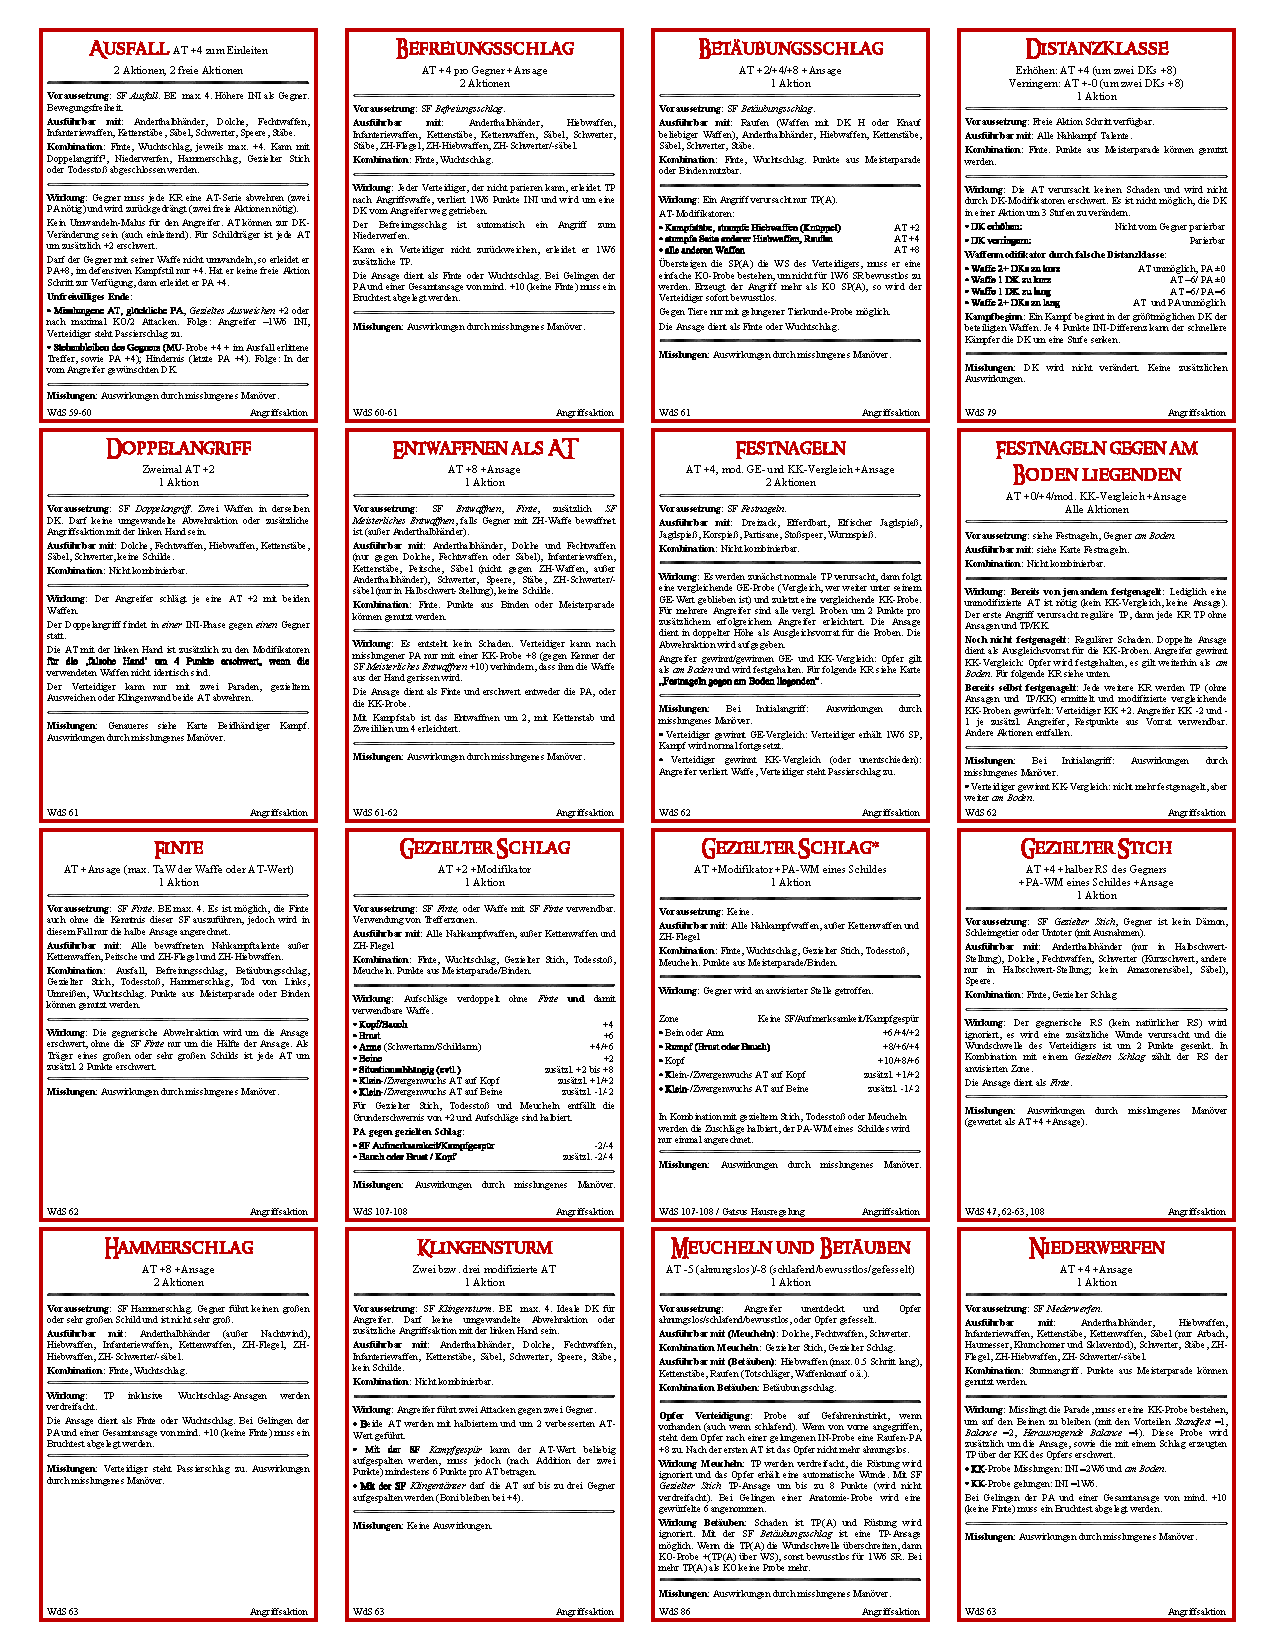
\includepdf[pages=-]{Kampf/Angriff/Angriffsaktionen.pdf}
    \phantomsection

    \addcontentsline{toc}{chapter}{Fernkampfmanöver}
    \hypertarget{fernkampfkarten}{}
    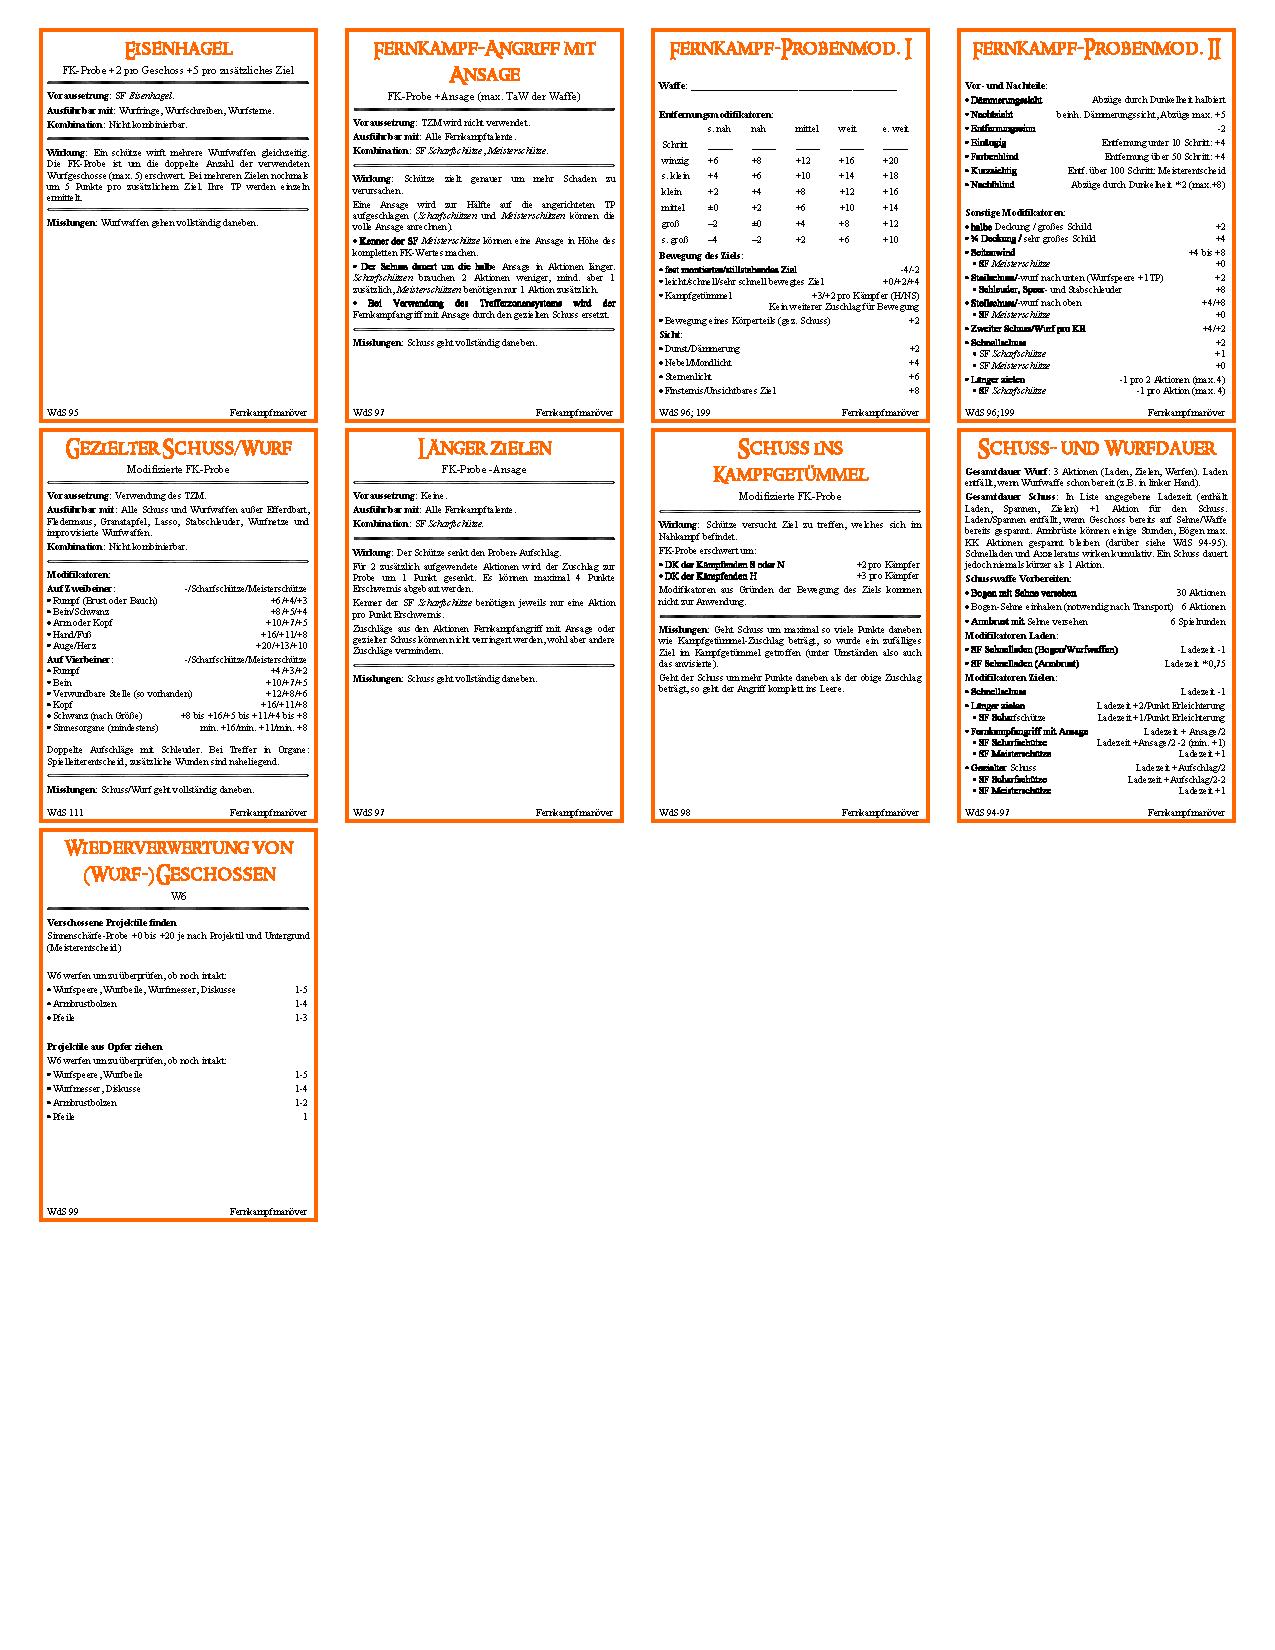
\includepdf[pages=-]{Kampf/Angriff/Fernkampfaktionen.pdf}
    \phantomsection

    \addcontentsline{toc}{chapter}{Waffenloser Kampf}
    \hypertarget{waffenloskarten}{}
    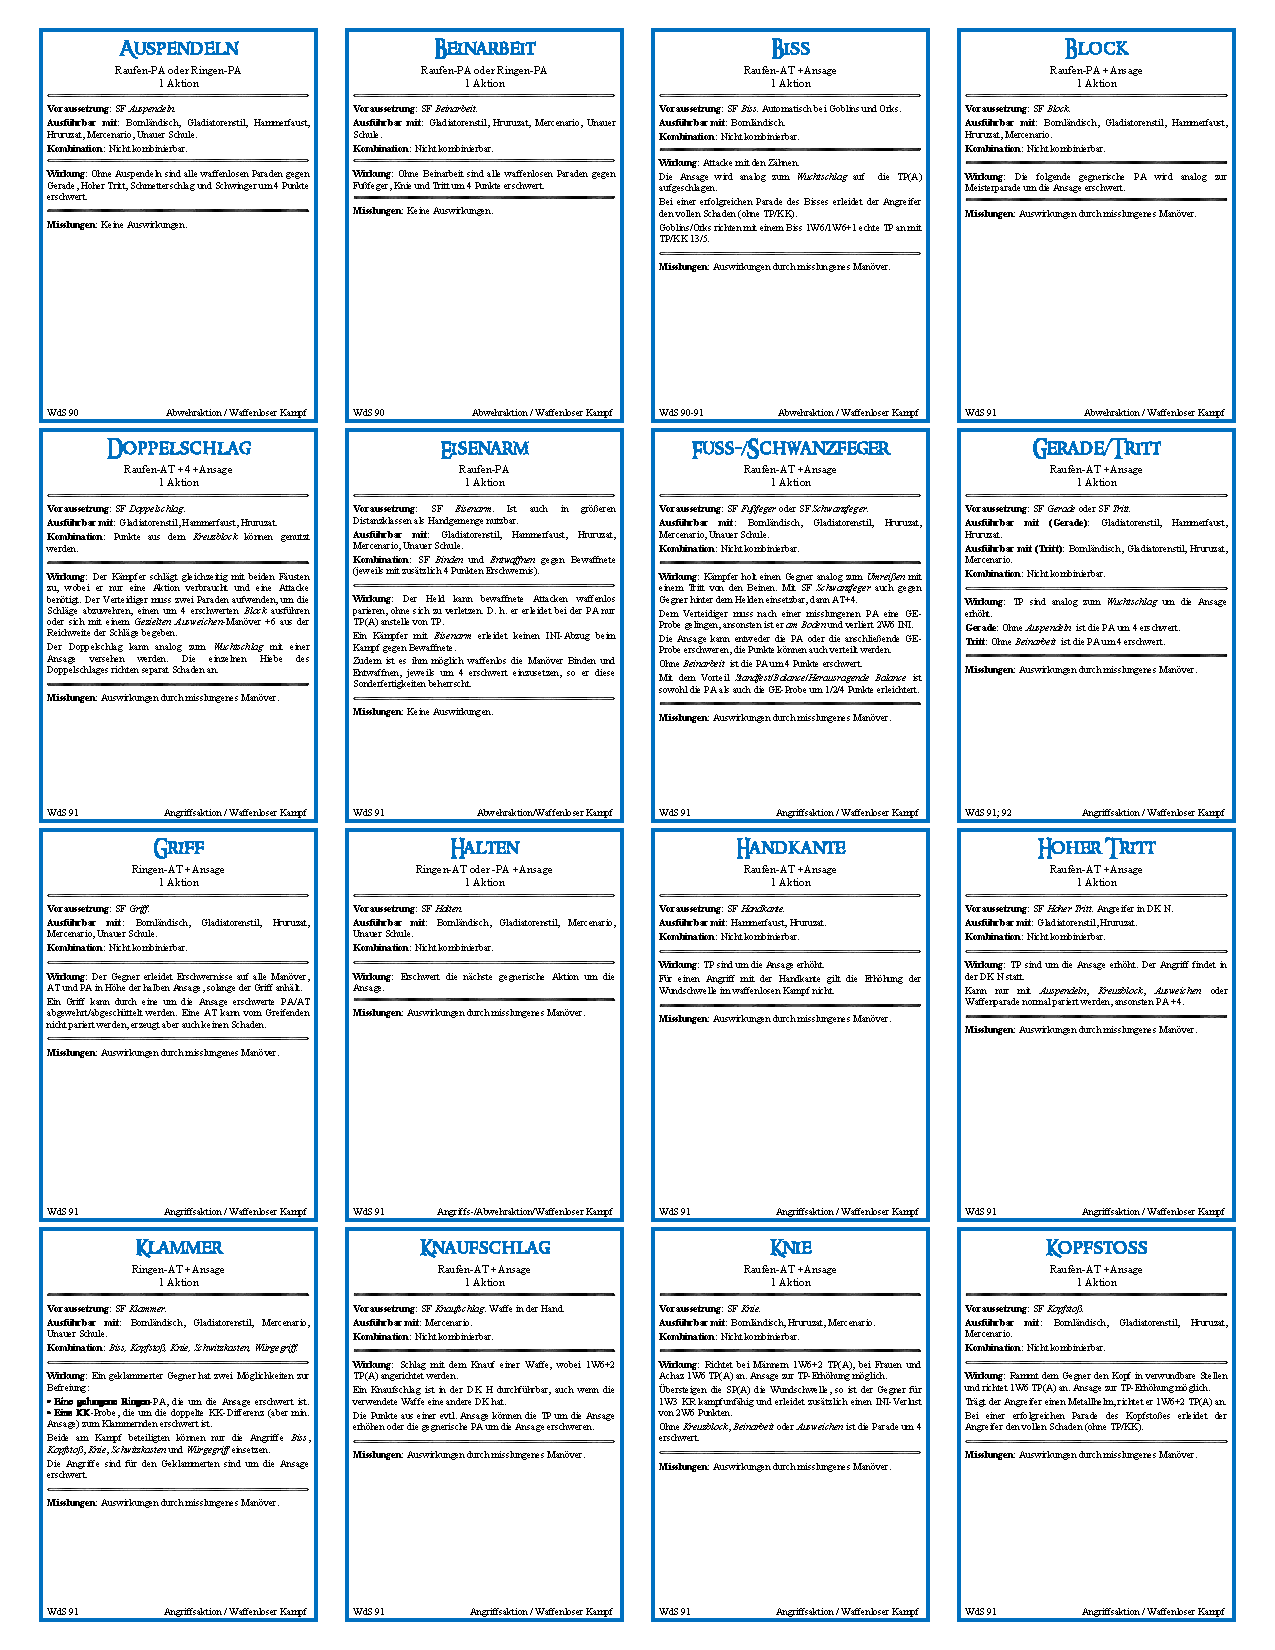
\includepdf[pages=-]{Kampf/Angriff/Waffenlos.pdf}
    \phantomsection

    \addcontentsline{toc}{chapter}{Parademanöver}
    \hypertarget{abwehrkarten}{}
    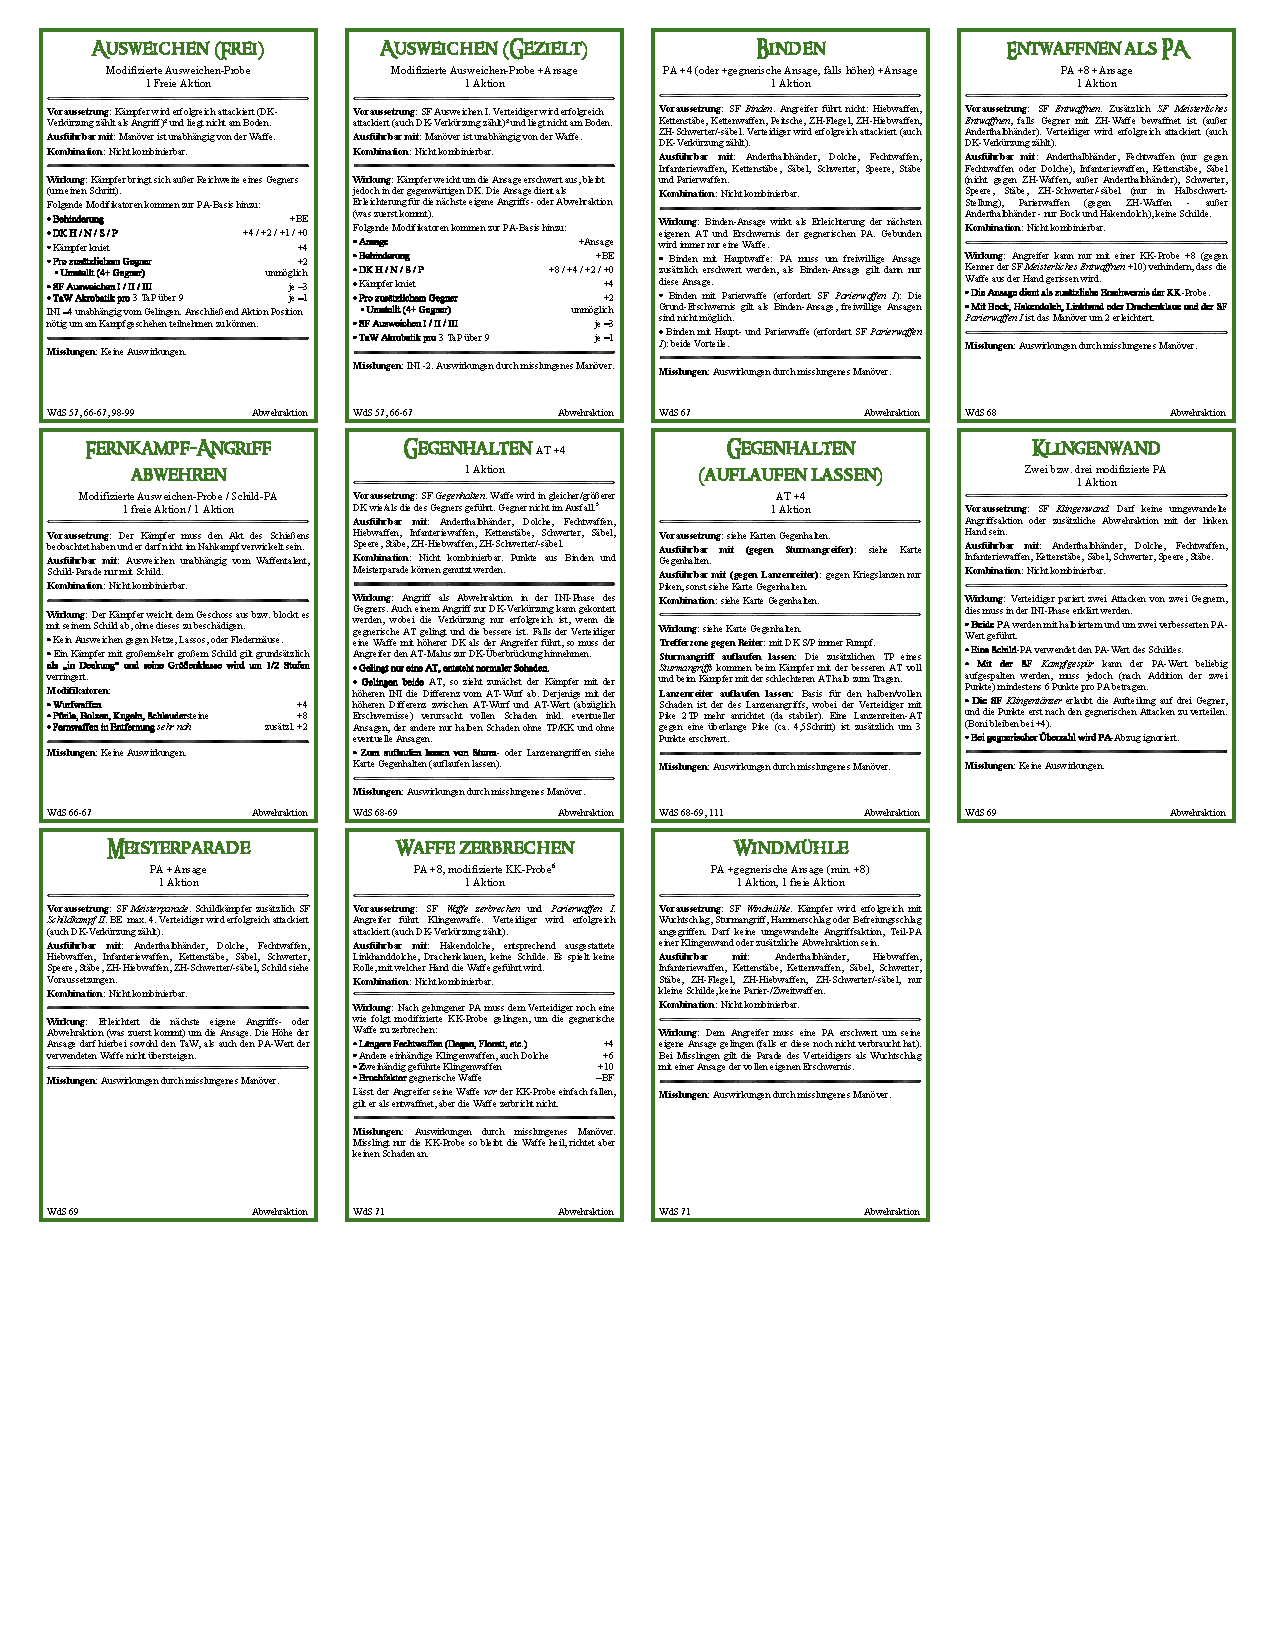
\includepdf[pages=-]{Kampf/Parade/Abwehraktionen.pdf}
    \phantomsection

    \addcontentsline{toc}{chapter}{Übersichtkarten}
    \hypertarget{übersichtkarten}{}
    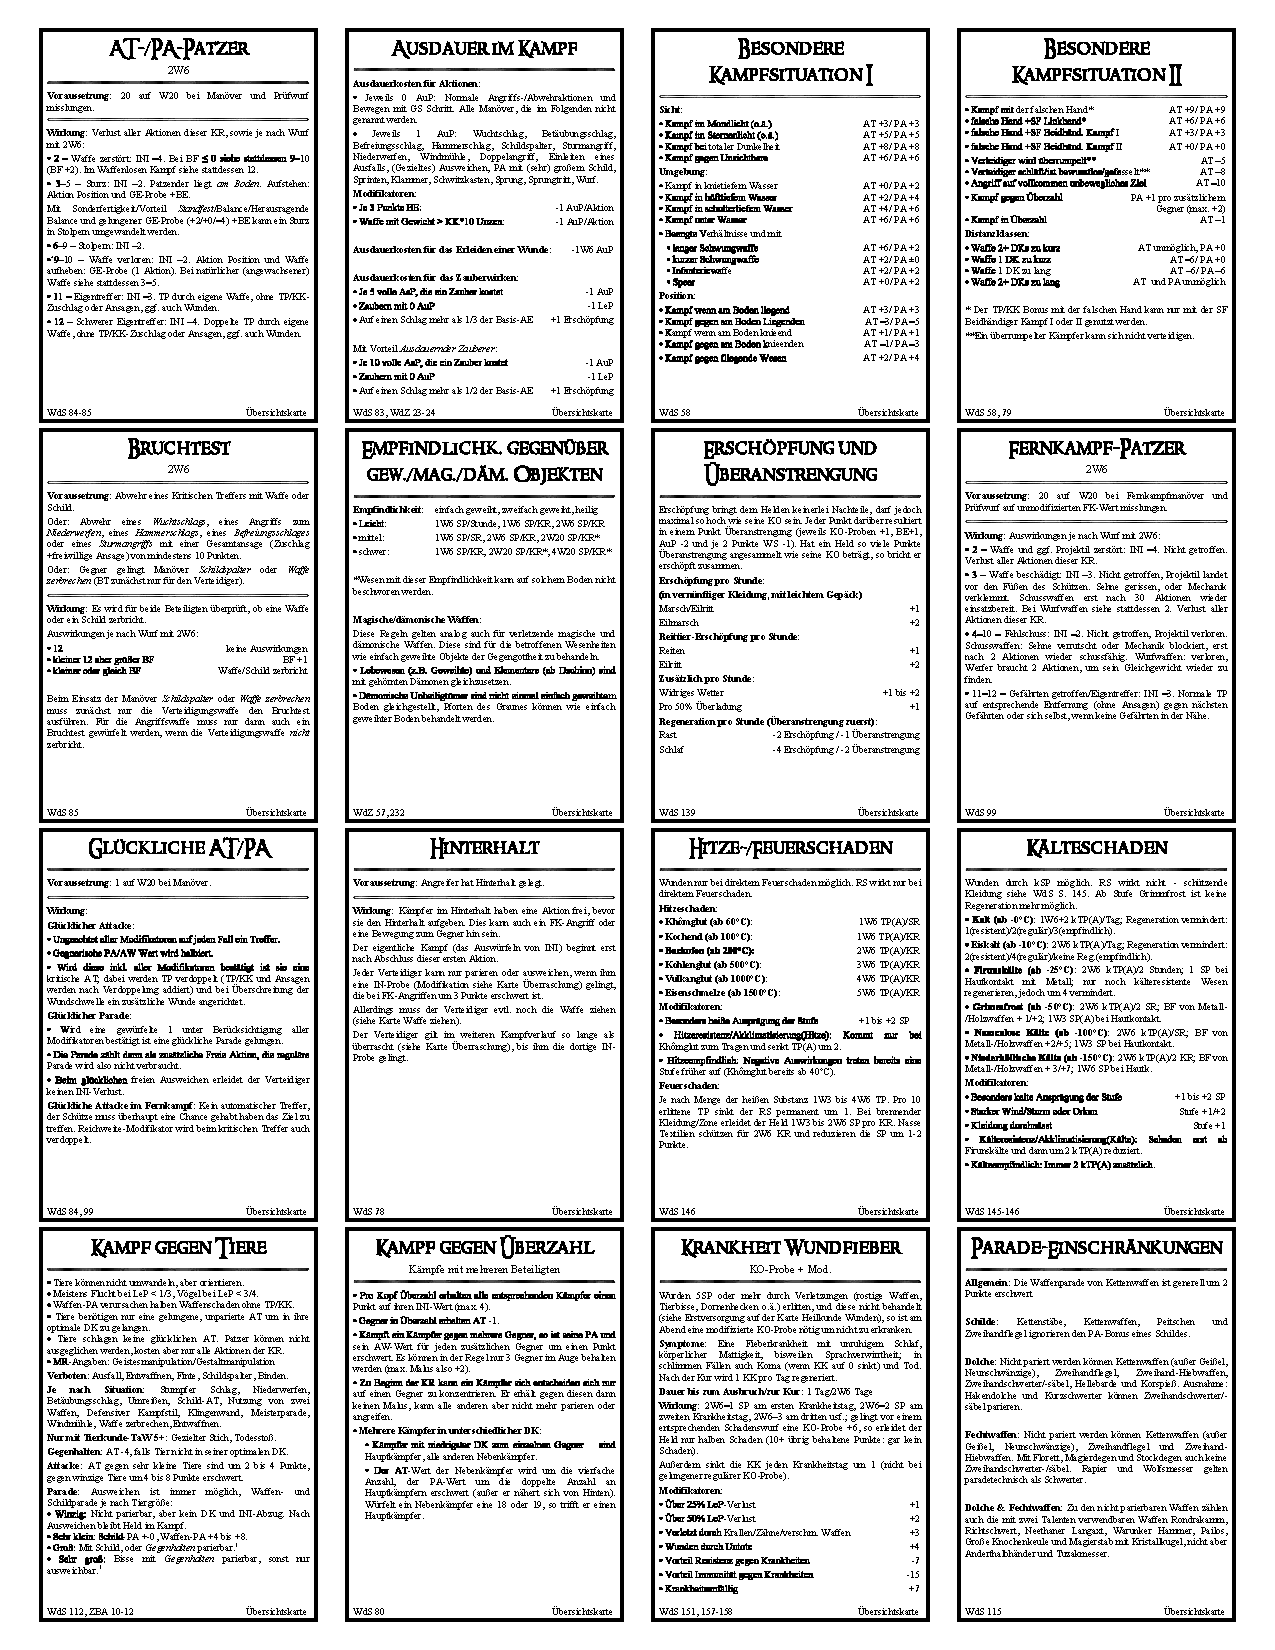
\includepdf[pages=-]{Kampf/Home/uebersicht.pdf}
    \phantomsection
\end{document}
